%===================================== CHAP 2 =================================

\chapter{Background Theory}

\section{Artificial Neural Networks}

\textit{This was missing in the specialization project. Need to cover all concepts used later in the report. This includes all different layers of a neural network. The layers (dropout, pooling, etc) could perhaps be a separate section after this one.}

\subsection{Biological Background}

The idea of an Artifical Neural Network (ANN) is that it can approximate any continuous function, and that it has the possibility of learning. ANNs are inspired by the structure and behavior of a biological brain and its ability to learn, but they are generally not intended to be realistic models. A neural network consists of interconnected nodes referred to as units. These correspond to a biological neuron, the basic computational unit of the brain, structured as illustrated in \textbf{Fig. \ref{fig1}}. The connections between the units corresponds to a biological neuron's dendrites, which provide input signals, and its single axon, which produces output signals and is connected to other neurons. \\

\begin{figure}
    \begin{minipage}{0.5\textwidth}
        \centering
            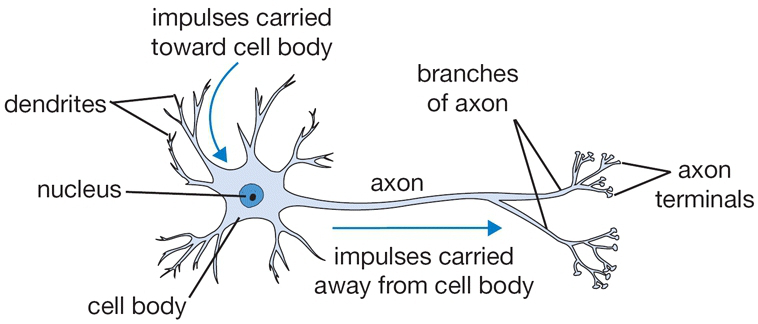
\includegraphics[width=1\textwidth]{fig/neuron}
            \caption{Biological neuron\cite{cs231n_part1}}
            \label{fig1}
    \end{minipage}
    \begin{minipage}{0.4\textwidth}
        \centering
            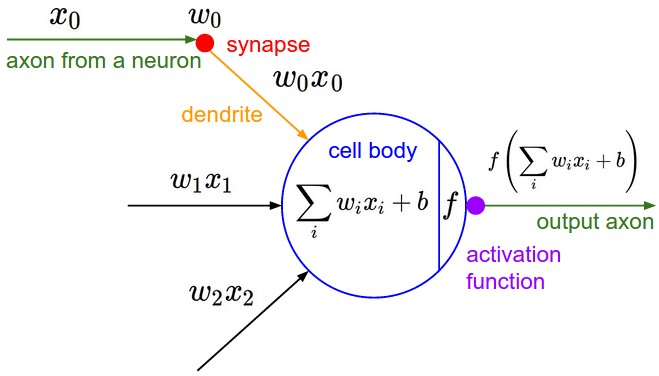
\includegraphics[width=1\textwidth]{fig/neuron_model}
            \caption{Mathematical model of a neuron\cite{cs231n_part1}}
            \label{fig2}
    \end{minipage}
\end{figure}

\noindent To simulate these signals, an ANN uses a mathematical model as illustrated in \textbf{Fig. \ref{fig2}}, where the signal is multiplied by the weight of a connection. The weight of a specific connection control how much the unit on one end influences the unit on the other end. The sum of all input signals are computed at the cell body of the unit. If this sum is above a certain threshold, the unit fires an output signal determined by its activation function by performing a specific mathematical operation on the sum.

\subsection{The Multi-Layer Perceptron}

\noindent The simplest form of an ANN is the single layer perceptron, which consists of only one layer of output nodes. This network can only learn linearly separable patterns. To allow for learning complex patterns, more layers need to be added, and we obtain the multi-layer perceptron (MLP). As layers are added, the depth of the network increases. This is why we refer to the the use of MLPs as "deep learning". \\

\noindent There are several different classes and types of ANNs. We will focus on the standard feed-forward neural network, and thus we will use the term ANN when referring to such a network. In this kind of network, all connections are directed from one layer to the next layer, and there are no cycles or connections between units in the same layer. \\

\noindent The first layer of an ANN is called the input layer. Similarly, the last layer is called the output layer. All layers in between are referred to as hidden layers, and are usually fully connected layers. This means that every node in a layer is connected to every node in the following layer. A hidden layer can also be a convolutional layer, or a pooling layer, but these cases will be covered in the section on convolutional networks.

\subsection{Activation Functions}

\noindent The common behaviour of all activation functions is that they define the output of a unit given a set of inputs. There are a great variety of activation functions in use, but we will only describe those most commonly used and thus considered in our implementation. The mathematical function of three of these are plotted in \textbf{Fig. \ref{activationfuncs}}. For further details we refer the reader to the Stanford CS class on convolutional neural networks\cite{cs231n_part1}. \\
\begin{figure}[H]
    \begin{minipage}{0.3\textwidth}
        \begin{tikzpicture}
            \begin{axis}[
                title = {Sigmoid function},
                axis lines = center,
                xtick={-10, -5, 5, 10},
                ytick={0, 0.2, 0.4, 0.6, 0.8, 1.0},
            ]
            \addplot [
                domain=-10:10,
                samples=100,
                color=blue,
            ]
            {1 / (1 + e^-x)};
            \end{axis}
        \end{tikzpicture}
    \end{minipage}
    \begin{minipage}{0.3\textwidth}
        \begin{tikzpicture}
            \begin{axis}[
                title = {Tanh function},
                axis lines = center,
                xtick={-10, -5, 5, 10},
                ytick={-1.0, -0.5, 0, 0.5, 1.0},
            ]
            \addplot [
                domain=-10:10,
                samples=100,
                color=blue,
            ]
            {(2 * (1 / (1 + e^-(2*x)))) - 1};
            \end{axis}
        \end{tikzpicture}
    \end{minipage}
    \begin{minipage}{0.3\textwidth}
        \begin{tikzpicture}
            \begin{axis}[
                title = {ReLU function},
                axis lines = center,
                xtick={-10, -5, 5, 10},
                ytick={2, 4, 6, 8, 1.0},
            ]
            \addplot [
                domain=-10:10,
                samples=100,
                color=blue,
            ]
            {max(0, x)};
            \end{axis}
        \end{tikzpicture}
    \end{minipage}
    \caption{The most commonly used activation functions}
    \label{activationfuncs}
\end{figure}

\subsubsection{Sigmoid}

The sigmoid activation function is mathematically defined as $\sigma(x) = 1/(1 + e^{-x})$. The function takes a number as input, and outputs a number within a continuous range from 0 to 1. It is commonly used as the activation function for the output node of a binary classification problem. Apart from this, the other activations functions tend to be preferred to the sigmoid function because of its drawbacks. The first drawback is that the outputs are not centered around zero, which can cause the network to display undesirable behaviour. A bigger drawback is that the activation saturates, meaning that the unit outputs mostly 0 and 1 instead of anything in between, and thus the gradient at these regions is very low. If the gradient falls to zero, the network will stop learning.

\subsubsection{Softmax}

The softmax activation function is a variant of the sigmoid function in that instead of being used in binary classification, it is used for the output nodes of a multiclass classification problem, where the goal is to classify instances into one of more than two classes. The mathematical equation for the softmax function is $f(x) = e^x/\sum_{j=0}^k e^{x_j}$. It calculates the probability distribution of each target class over all possible target class. A convenient result of this is that the sum of all probabilities will be equal to one. Note that the softmax function is not used in middle nodes, but only as the activation function of output nodes.

\subsubsection{Tanh}

The tanh activation function is a scaled version of the sigmoid function. Its mathematical function is $tanh(x) = 2\sigma(2x) - 1$. The scaling causes the tanh function to output numbers within the range of -1 and 1. This makes the output zero-centered, thus avoiding the first drawback of the sigmoid function. Even though the tanh function still stuffers from saturation, it is preferred to the sigmoid function.

\subsubsection{ReLU}

The Rectified Linear Unit (ReLU) activation has the mathematical function $f(x) = max(0,x)$. This means that it is very close to linear; thresholding the input at zero, but keeping any value above. It has become very popular, and is in general the activation function of choice. It is non-saturating, and has been found to speed up the convergence of the learning. The computation of the function is also very inexpensive compared to the sigmoid and tanh function. The only problem with the ReLU function is the possibility of "dead" units, meaning that they will never activate. Generally, adjusting the learning parameters can prevent this, but there have also been several attempts to fix this issue, for instance using so called PReLU or Maxout units.

\subsection{Training a Network}

The weights of a model can be learned by training the model on a set of input and output values, a task which is called supervised learning. There are also other kinds of learning, but we will not cover these. The learning process runs for a number of epochs, meaning the number of times the learning algorithm will see the entire data set. Often, the data is split into so-called batches when passed to the algorithm. The number of training examples in a batch is referred to as the batch size.

\subsubsection{Loss Function}

\noindent The goal of an ANN is to find a function that solves a certain problem, more specifically that finds an optimal solution to the problem. The definition of this optimal solution is that given a loss function, there are no other solution with less of a loss. The loss function is in that sense a measure of how far away a solution is from an optimal solution. The goal of the learning process is thus to find a function with the smallest possible loss. The weights of a model can be learned by training the model on a set of input and output values, a task which is called supervised learning. There are also other kinds of learning, but we will not cover these. In supervised learning, the goal is to find the function that best maps the input to the output. The loss will then be the mismatch between such a mapping and the example data.

\subsubsection{Vanilla Gradient Descent and Backpropagation}

\noindent To optimize the loss, we can use an algorithm called gradient descent, which minimizes any function iteratively. The process is a repeated loop of evaluating the gradient, and then updating the weights based on this gradient. The simplest form of this algorithm, also called its vanilla version, is shown in \textbf{Code \ref{code:1}}.

\begin{listing}%[ht]
\begin{minted}
[
frame=lines,
framesep=2mm,
baselinestretch=1.2,
fontsize=\footnotesize,
linenos
]
{python}
for i in range(epochs):
    weights_grad = evaluate_gradient(loss_function, data, weights)
    weights += - learning rate * weights_grad
\end{minted}
\caption{Vanilla gradient descent}
\label{code:1}
\end{listing}

\noindent First, the algorithm evaluates the gradient of the loss function for the whole data set with respect to the current weights. This is done using an algorithm called backpropagation. Often, the term is used to refer to the complete process of repeatedly computing the gradient and updating the weights. Each iteration of computing the gradient involves two steps: forward propagation and backward propagation. The forward propagation is simply the propagation of an input through the network in order to generate an output. In the backward propagation, the loss, or error, between the generated output and the actual output is computed, and this error is propagated backwards to the previous layers. The error values are then used to calculate the gradient. The next step of gradient descent is to adjust the weights, based on the evaluated gradient and a learning rate. The learning rate controls the magnitude of the update, and is a crucial network hyperparameter setting. This process is repeated for a pre-defined number of epochs.

\subsubsection{Stochastic Gradient Descent}

The vanilla version of gradient descent is also called batch gradient descent. A batch of data is a portion of the training data, in this case the entire training data set. The gradient is computed over such a batch, which is very slow and expensive in terms of memory. There are a number of different ways to optimize gradient descent by extending its vanilla version. Stochastic gradient descent (SGD) is one of these methods. In this case, the gradient is computed over mini-batches consisting of only one training pair. This is a special case of the more general mini-batch gradient descent, which computes the gradient over batches of the training data, instead of the entire set. SGD refers to both mini-batch gradient descent, as well as the special case of stochastic gradient descent. Usually it is more efficient to compute the gradient over a number of examples instead of only one. Even though SGD is much more efficient than the vanilla version, it also has its drawbacks, and therefore a number of algorithms intended to improve this has been developed.

\subsubsection{Adding Momentum}

One way to improve SGD is to add momentum. SGD can get stuck in local optima, and adding momentum can help accelerating in the right direction. A further improvement is the Nesterov momentum, which adds some notion of where SGD is heading by approximating the next position.

\subsubsection{Adaptive Learning Rate Methods}

Adaptive learning rate methods are algorithms that automatically adapts the learning rate to the parameters. They are quite similar, and perform thereafter. In general, SGD often finds a minimum, but these methods can help to achieve faster convergence, and you do not have to tune the learning rate. The algorithms are usually implemented with a good default starting value. Adagrad was the first adaptive learning rate method proposed, and the others are thus extensions to this. Its weakness is that the learning rate decreases and eventually becomes close to zero. Adadelta and RMSprop are methods that try to overcome this, and they are close to identical. Adam adds some form of momentum to the optimization, and therefore might be the best overall choice.

\subsubsection{Regularization}

Dropout, L2 regularization, etc.

\section{Convolutional Networks}

\textit{More in-depth than covered in the specialization project. \\
What exactly is the convolutional operation? Convolutional layer (local connections and weight sharing) vs normal layer.}

\begin{itemize}
    \item Convolutional layer
    \item Pooling
\end{itemize}

\section{Visualization}
\textit{Describe all the different techniques, perhaps in more detail. \\
Possibly even implementation level.}

\subsection{Why Visualize?}

When using ANNs to solve complex problems, like face recognition, it is not unlikely that the network requires millions of parameter values to obtain a desirable performance level. In these cases, it is hard to gain insight about the network's performance by examining the parameter values directly, both because of the unfeasible amount of values and each value's relative insignificance. However, when applying ANNs to tasks in the image domain, there are several ways to help us understand the inner workings of the network by presenting information in the same readable format as the input. Aside from the fact that images more suited than numbers for human readability, there exists several techniques that utilizes the connections in the network to produce visualizations. These images can then provide insight into a larger part of the network, spanning several layers, possibly the whole network. Through the use of these visualization techniques, the network can improved by making informed decisions, instead of employing a trial and error approach.

\textit{Visualization offers a reasonable method for presenting the vast amount of information available when analyzing a convolutional neural network in a readable manner. For example, one technique allows us to view which areas of an input image a classifying network focuses on, informing us on what the network discerns as important when computing output classifications}. \\

\noindent \textit{To gain a beneficial amount of information from our visualization website, we determined several different techniques to be researched. In this section, we present the techniques we have selected as appropriate for our purpose. Their advantages and relevance are discussed, and a brief description of how they function are given. For further explanations on implementation, we refer the reader to their respective articles.} 

\subsection{Training Progress Measurements}

Throughout training, the progress of the network is visualized in a simple line plot. Measurements are made of the standard network appraisal values, loss and accuracy, both on the training set data and, if provided, the validation set data. A typical thing to want to monitor, these values provide a means to explicitly evaluate a network’s performance. Plotting the values against time, at certain batch intervals or at epoch completion, puts the current measurements in perspective, and makes the training progress, or lack thereof, easily discernible. The shape of the line plot could also be used to reveal undesirable values in the training hyperparameters. For example, if the learning rate is too large, the network is likely to vastly improve at first, only to have its progress quickly stagnate. In this case, both loss and accuracy plots would have distinct shapes that indicate a problem, without having to look at any of their actual values.

By including the validation values, one could also be able to identify the presence of overfitting, marked by a point where the validation accuracy begins to decline while training accuracy continues to rise.

\textit{The training progress measurements include standard network appraisal values, like loss and accuracy on the training set data, and the loss and accuracy of the validation set data, if provided. It is a typical thing to monitor, and provides a means to explicitly evaluate a network’s performance. Plotting these values against time, for example at each batch or epoch completion, puts the current measurements in perspective, and makes the training progress, or lack thereof, easily discernible. By including the validation values, one could also be able to identify the presence of overfitting, marked by a point where the validation accuracy begins to decline while training accuracy continues to rise.}

\subsection{Layer Activations}

\textit{The activation output is most readable for the convolutional layers, and especially so for the earlier ones. The activations in convolutional layers can also be called feature maps, and the units in these maps typically share the same weight matrix, called the filter. The filter will, through backpropagation, learn to look for certain features, for example a horizontal edge. Applying the filter to the input creates the feature map, which can convey information about where the filter found the feature it was looking for. For deeper convolutional layers, these features become more complex and so does the input. It is the simplicity of their filters and input that make the earlier layers activations easier to interpret. Considering these filters, the activation output can be helpful to confirm that the network is progressing well, if the output is showing signs of activation in areas with similar features. These patterns should become more and more clear as training goes on, and when the activations start experiencing little or no change, the proper filters should be obtained.} \\

\noindent \textit{Additionally, in networks using ReLUs, a common activation function, the expectation of seeing sparse and localized activations can be confirmed, which is an indicator of the network learning properly. If some feature maps are entirely dark, with all pixel values zero, this can be a warning sign that the learning rate is too high. The particular filters are then rendered useless, and they have no possible way to recover \cite{cs231n_act}. }

\subsection{Saliency Maps}

\textit{A salience map is typically a black-and-white image with the same size as the input, where important pixels have a high value, and insignificant pixels have a low value \cite{salience}. Thus, the important regions can be easily identified by their brightness. A map for classification is specific to an image and a class, and it allows us to observe which parts of an image influences the network classification score the most. In other words, we can view which parts of an image that the network deems more important when deciding upon the classification score chosen. Such a map can be produced by efficiently using the back-propagation gradient of the output score with respect to the input image.} \\

\noindent \textit{In a face recognition case, the saliency would allow us to investigate what the network emphasizes, for example which facial regions are decisive in producing the identification output. We could also exploit salience maps for expression classification, creating maps to display which areas were the most influential for selecting the outputted expression results. By using the insight gained through salience maps, we would be able to confirm our beliefs that a network focuses on regions containing important feature information, and alert us to any peculiarities.}

\subsection{Deconvolution Network}

Modern networks that receive images as inputs are likely to have convolutional layers form the initial part of the network. This part is aimed at detecting certain features in the image, with the complexity of the features rising as the depth of the convolutional part increases. In such cases, we can utilize a visualization technique that employs a deconvolutional network, which can be thought of as a reverse convolutional network \cite{deconv_net}. The visualizations are used to interpret the feature activity in the intermediate layers of the original network. To obtain a visualization, an image is first fed to the original network to produce activations in its various layers. The activations of the convolutional part can then be processed and fed to the deconvolutional network to create a visualization of the pattern in the input image that was responsible for eliciting the given activations. This pattern can then reveal what a certain part of the original network finds important and what it is looking for in an image. \\

\noindent To build such a deconvolutional network, it is necessary to examine the original network we want to produce visualization for. Only the feature extracting part is of interest, and we can regard this part as a network on its own. The purpose of the deconvolutional network is to map the feature activity present in this convolutional network back to the input pixel space \cite{deconv_vis}. For a convolutional network consisting of convolution and max pooling layers, the corresponding deconvolutional network would consist of transposed convolution and unpooling layers in the opposite order of the original layers. In addition, where a ReLU activation function commonly follow each convolution layer, they would precede transposed convolution layers. In other words, by a top-down examination the convolutional network would enable a bottom-up creation of the deconvolutional network. \\

\noindent A transposed convolution layer (also known as a fractionally strided convolution layer) is used to reverse the convolution layer effects. Where as a convolution layer typically performs downsampling, i.e. it outputs matrices that have dimensions smaller than the ones it receives as input, a transposed convolution typically performs upsampling, i.e. it outputs matrices that have dimensions greater than the ones it receives as input. To achieve this, a transposed convolution swaps the forward and backward passes of a convolution, both of which can be defined by the kernel. Consider a 3x3 kernel used in a normal convolution on a 4x4 matrix. If we unroll the matrix from left to right and top to bottom, the convolution can be represented by the matrix $C$, where \textit{$w_{ij}$} is the element at row \textit{i} and column \textit{j} in the kernel:

\[
    C = 
    \left(
    \begin{smallmatrix}
    \textit{$w_{00}$} & \textit{$w_{01}$} & \textit{$w_{02}$} & 0 & 
    \textit{$w_{10}$} & \textit{$w_{11}$} & \textit{$w_{12}$} & 0 & 
    \textit{$w_{20}$} & \textit{$w_{21}$} & \textit{$w_{22}$} & 0 & 
    0 & 0 & 0 & 0\\
    0 & \textit{$w_{00}$} & \textit{$w_{01}$} & \textit{$w_{02}$} & 
    0 & \textit{$w_{10}$} & \textit{$w_{11}$} & \textit{$w_{12}$} & 
    0 & \textit{$w_{20}$} & \textit{$w_{21}$} & \textit{$w_{22}$} & 
    0 & 0 & 0 & 0\\
    0 & 0 & 0 & 0 & 
    \textit{$w_{00}$} & \textit{$w_{01}$} & \textit{$w_{02}$} & 0 & 
    \textit{$w_{10}$} & \textit{$w_{11}$} & \textit{$w_{12}$} & 0 & 
    \textit{$w_{20}$} & \textit{$w_{21}$} & \textit{$w_{22}$} & 0\\
    0 & 0 & 0 & 0 & 
    0 & \textit{$w_{00}$} & \textit{$w_{01}$} & \textit{$w_{02}$} & 
    0 & \textit{$w_{10}$} & \textit{$w_{11}$} & \textit{$w_{12}$} & 
    0 & \textit{$w_{20}$} & \textit{$w_{21}$} & \textit{$w_{22}$}\\
    \end{smallmatrix}
    \right)
\]

\noindent Multiplying $C$ with the now 16-dimensional vector would produce a 4-dimensional vector, which could be reshaped into the 2x2 matrix we expect from the convolution. The operation is therefore equivalent to a convolution forward pass. To do a convolution backward pass, the transposed version of $C$, $C^T$, would be used. This transposed version of the convolution matrix allows the backward pass to receive a 4-dimensional vector as input and produce a 16-dimensional vector as output, which can be reshaped to the original 4x4 size. \\

\noindent In a forward pass, a single entry in the output vector is only affected by a subset of the entries in the input vector and always the same ones. The backward pass has the same connectivity pattern between the entries in the input and output vector, only in the reverse order. These connectivity patterns are compatible since both passes are defined by $C$. In context of the example, the first entry (index 0) of the forward pass output vector would be connected to the input vector entries with index 0-2, 4-6, and 8-10. Subsequently, the backward pass output vector entries with index 0-2, 4-6, and 8-10 would be connected to the first entry in the input vector.\\

\noindent Where a normal convolution uses $C$ and $C^T$ for the forward and backward pass, respectively, the transposed convolution would use $C^T$ and $C$ for the forward and backward pass, respectively. As $(C^T)^T=C$, the transposed convolution is simply a convolution using transposed convolution matrices, hence the name. Because both the passes in transposed convolution are defined by $C$ as well, the connectivity pattern found in normal convolution also holds for transposed convolution. \\

\noindent The fact that a transposed convolution can reverse a convolution downsampling while maintaining a similar connectivity pattern makes them suitable for a deconvolutional network. A convolution layer in the original network would apply their filters to the output of the previous layer (or the image input) and produce feature maps, which are then rectified by the ReLU activation function. In the deconvolutional network, the aim is to map the rectified feature maps back to convolution input, and this is where transposed convolution is used. By using the same filter weights in a transposed convolution layer as in its corresponding convolution layer, the deconvolutional network is able to create a mapping that is specific to the original network. \\

\noindent As previously mentioned, the input to the transposed convolution should first be passed through a ReLU activation function. In a convolution layer, ReLU ensures that the feature maps outputted are strictly positive. For the convolution input reconstruction to be valid, the reconstructed feature maps used as input for the transposed convolution layers must also be strictly positive. Passing the reconstructed feature maps through a ReLU activation function ensures this. \\

\noindent To reverse the effects of the max pooling layers of the original network, the deconvolutional network uses unpooling layers. Pooling, however, is not an invertible operation and the unpooling layers therefore focus on obtaining an approximation of the original max pooling input. The key to the approximation is to use a switch variable for each pooling region. When performing max pooling, these switches record the location of the chosen maximum in each region and pass the information to the unpooling layer. Here, they are used to place the entries in the unpooling input into the appropriate locations in the output. The result is an unpooling output that only has non-zero values in entries that correspond to the maximum entries in the pooling input. This reconstruction approach preserves the structure of how max pooling processes stimulus. \\

\noindent To utilize a constructed deconvolutional network, first the feature map output from a chosen layer in the original network must be produced. Before the feature maps are fed to the corresponding layer of the deconvolutional network, they must be processed. To visualize what a particular filter is looking for, all entries in the feature maps is set to zero, except the maximum entry in the filter's corresponding feature map. Only the maximum entry is left untouched to create a visualization that is able to convey what pattern in the input image activates that filter strongly. When the processed feature maps are inputted into the deconvolutional network, the layers will successively reconstruct the activity that was responsible for the chosen feature map activation until the input pixel space is reached. If visualizations for several filters are desired, the deconvolutional network has to run multiple times, each with feature maps only containing a single non-zero entry. \\

\noindent When the original network is applied to an input image, the switches created in its max pooling layers are specific for that image. The reconstruction from the processed feature maps are created using these switches and it will therefore resemble the input image. However, only the patterns that contribute towards the chosen feature map activation are reconstructed. The visualization outputted by the deconvolutional network will then be mostly blank, with a highlight of the important section of the image and its characteristics. Creating visualizations from several images for a single filter can reveal what the filter is looking for. For example, if a filter is trained to detect eyes, the reconstructions from this filter will repeatedly focus on image sections containing eye-like traits, as well as highlighting those traits. One could also have a single image and use several different filters to produce visualizations, which could reveal if the original network is capable exploiting the discriminative features in the image. If a network is supposed to locate faces, but none of the visualizations show any focus on the eyes, they could warn about flaws in the network and potentially explain poor performance. Conversely, if the visualizations cover a wide range of facial characteristics, they can provide reassurance about the quality of the network's feature utilization. \\

\noindent Visualizing for several layers can also shed light on the hierarchy of the filters, where the lower layers usually concentrates on low level features like edges and textures and the upper layers looks for more complex features, e.g. eyes. If a network experiences problems with upper layer filters, it is possible that these stem from poor filters further down. Applied during training, visualizations from different layers reveal when the filters of each layer converges. Typically, the lower layer filters converge quickly, while the upper layer filters develop at a much slower rate.


\subsection{Deep Visualization}

In contrast to the other techniques discussed, deep visualization does not require any input image...

\subsubsection{$L_2$ Decay}

Employing $L_2$ decay is a common regularization technique for ANNs, where it is used to penalize large weight values. In these cases, the weights are linearly decayed towards zero with a chosen regularization strength. In deep visualization, $L_2$ decay is similarly applied to the input image, where it is used to penalize extreme pixel values and prevents them from dominating the image. This is desirable as extreme pixel values are neither naturally prevalent nor useful for visualizations.

\subsubsection{Gaussian Blur}

Without regularization, the image generated from deep visualization has a tendency to contain a great deal of high frequency information, i.e. the pixel values are often radically different from that of their neighbours. While normal images do contain some high frequency information, for example at edges of objects, an excessive amount of it leads to unrealistic and uninterpretable visualizations. 

Induced by the gradient ascent for its ability to cause high activations in the network, this high frequency information impedes the image's visualization qualities. 

\subsubsection{Clipping Based on Value}



\subsubsection{Clipping Based on Norm}



\subsubsection{Clipping Based on Contribution}
Explain both abs. and normal contribution...

\textit{Deep visualization offers visualization of the learned features of a network, computed by the individual neuron at each layer \cite{deepvis, deepvis_web}. The outputs are images that maximally activate individual neurons, and represent what the neurons in the network have learned to look for. Starting with random images, the method iteratively updates the images based on the gradient update of a chosen neuron to create images that optimally triggers the activation of that neuron. For example, in an image classification network, we could use the output neuron responsible for the class ‘cat’, and produce deep visualizations for this neuron. The resulting images should display various catlike features across their pixel space. As we start with random images, the optimization is stochastic, meaning that the variance of these images provides information about the network unit’s learned invariances. In our case, we could choose neurons that classify the face recognition result to similar effect. If the neurons are looking for sensible features, the network is heading in the right direction. If the features portrayed are irrational or intangible, the opposite might be the case.} \\ 

\noindent \textit{The visualization is not restricted to the output units, and can be performed for all neurons in the network. We can then determine what a hidden unit has learned to look for, which would typically be a lower level feature. For very low layers, this could for example be edges. In the face recognition domain, at an intermediate layer, we might get output images depicting an eye, or eyelike features.} \\

\noindent \textit{It is important to note that the technique is reliant on heavy regularization to produce recognizable and interpretable output images.}

\section{Transfer Learning}

\section{Face Recognition}

\textit{Can probably use a lot from the specialization project here.}

\section{Facial Expression}

\textit{Here as well.}

\cleardoublepage